\section{Toolkit Overview}

\begin{figure}
\centering
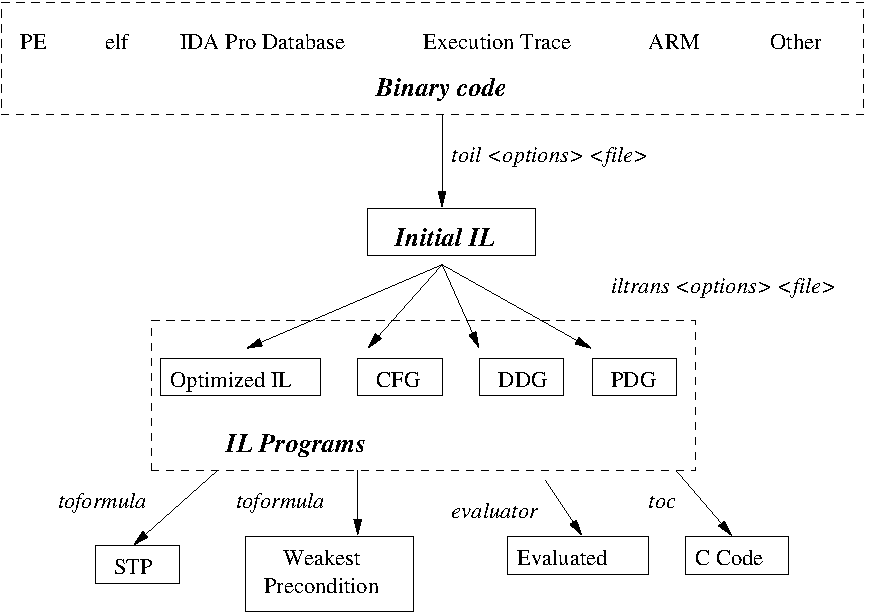
\includegraphics[scale=.8]{fig/toolchain}
\caption{High-level view of tools provided with \bap.}
\label{fig:toolchain-overview}
\end{figure}

There are several tools built and distributed with \bap. First, we
provide a tool called {\tt toil} which lifts binary code to \bil.
Second, we provide a tool called {\tt iltrans} which takes as input
\bil code, transforms it, and then outputs the resulting \bil
code. Thus, {\tt iltrans} is a mapping from \bil to \bil.  Finally, we
provide a set of additional utilities such as one that evaluates \bil
programs, and another that calculates the weakest precondition for a
\bil program. Figure~\ref{fig:toolchain-overview} shows the
relationship of these tools.  Different output options include
optimizing the IL, generating CFG's, PDG's, DDG's, and CDG's,
calculating the weakest precondition, and several other options. We
describe these tools at a high level in this chapter. 

{\tt Note:} Each tool provides a {\tt -help} option, which provides
the latest set of command-line options.







